\documentclass{article}

\usepackage{amsthm}
	\newtheorem*{definition}{Definition}
	\newtheorem*{theorem}{Theorem}
	\newtheorem*{lemma}{Lemma}
\usepackage{amsmath}
\usepackage{amsfonts}
\usepackage[margin=1in]{geometry}
\usepackage{hyperref}
\usepackage{tikz}
	\usetikzlibrary{cd}
	\usetikzlibrary{patterns}

\title{\href{https://math.umn.edu/sites/math.umn.edu/files/exams/mantopf19.pdf}{Fall 2019 Manifolds and Topology Preliminary Exam}}
\author{University of Minnesota}
\date{}
\begin{document}
\maketitle

\section*{Part A}
\begin{enumerate}
	\item Give a precise definition of the product $\alpha * \beta$ of two paths in a space $X$, including the conditions under which it is defined.
	
	\begin{definition}
	Let $\alpha, \beta: [0,1] \rightarrow X$ be continuous functions into $X$. If $\alpha (1) = \beta(0)$, then the product
	$\alpha * \beta: [0,1] \rightarrow X$ is defined to be 
	\[ (\alpha * \beta ) (t) = \begin{cases} \alpha(2t) & t \in [0,1/2] \\  \beta(2t-1) & t \in (1/2,1]\end{cases}\].
	\end{definition}
	
	\item Suppose that $X$ is a path connected, semilocally 1-connected space whose fundamental group is $\mathbb{Z}/2 \times \mathbb{Z}/2$. How many isomorphism classes of connected covering spaces does $X$ have?
	
	% See Hatcher prop 1.38
	\begin{proof}
		The isomorphism classes of covering spaces correspond to conjugacy classes of the fundamental group. 
		Thus, this question is equivalent to counting the conjugacy classes of $\mathbb{Z}/2 \times \mathbb{Z}/2$.
		Note that $\mathbb{Z}/2 \times \mathbb{Z}$ is abelian and abelian groups have exactly one conjugacy class for each group element (since $h g h^{-1} = h h^{-1} g = g$ for any $g,h$).
		Thus, there are $|\mathbb{Z}/2 \times \mathbb{Z}/2| = 4$ conjugacy classes, and hence there are $4$ isomorphism classes of covering spaces of $X$.
	\end{proof}
	
	\item Give an example of a space $X$ with open subsets $U,V$ such that $X = U\cup V$, $U$ is simply connected, $V$ is simply connected, but where $X$ is not simply connected. 
	Then explain why this does not violate the Siefert-van Kampen theorem. 
	
	\begin{proof}
		Let $X$ be the annulus of inner radius $1$ and outer radius $2$, shown below,:
		
		\begin{center}
                    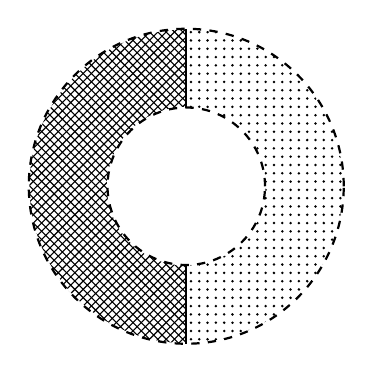
\begin{tikzpicture}
                    	\filldraw[pattern=dots,draw=white] (0 ,-1) arc [radius=1, start angle=-90, delta angle=180]
                  				-- (0,2) arc [radius=2, start angle=90, delta angle=-180]
                 				 -- cycle;
				 
			\filldraw[pattern=crosshatch, draw=white] 
						(0,1) arc [radius=1, start angle=90, delta angle=180]
                  				-- (0,-2) arc [radius=2, start angle=-90, delta angle=-180]
                 				 -- cycle;
				 
			\draw[thick] (0,1) -- (0,2);
			\draw[thick] (0,-1) -- (0,-2);
                    	\draw[thick, dashed] (0,0) circle (2cm);
			\draw[thick, dashed] (0,0) circle (1cm);
		
                    \end{tikzpicture}
                    \end{center}
                    and let $U$ be the closed left half of the annulus (shown crosshatched) and let $V$ be the closed right half of the annulus (shown filled with dots), where both $U, V$ include the line segments $\ell_+ = [(0,1),(0,2)]$ and $\ell_-=[(0,-1),(0,-2)]$.
                    
                    Then $\pi_1(U) = \pi_1(V) = 0$ since both are contractible. Additionally, $\pi_1(U \cap V) =  0$ since both the line segments $\ell_+, \ell_-$ are contractible so regardless of choice of basepoint we are in a contractible connected component. $U$ and $V$ do not violate the hypothesis of the Siefert-van Kampen theorem, because the intersection $U \cap V$ is not path-connected, however if it did, the theorem would tell us that $\pi_1(X) = 0/0 \cong 0$.
                    
                    On the other hand, we know that $\pi_1( U \cup V) \cong \mathbb{Z}$ because the generators are the trivial loop and the loop which contains the hole in its interior.
                    
                    Thus, we cannot choose $U,V$ as in this example if we wish to use the Siefert-van Kampen theorem.
	\end{proof}
	
	\item Explain why the inclusion $\mathbb{R}^2 - \{0\} \rightarrow \mathbb{R}$ is not a covering map.
	
	% See Hatcher prop 1.31
	\begin{proof}
		Suppose $\iota : \mathbb{R}^2 - \{ 0 \} \rightarrow \mathbb{R}$ were a covering map. 
		
		Then it is a theorem that the induced map $\iota_*: \mathbb{R}^2 - \{ 0 \} \rightarrow \{ 0 \}$ is an injection. 
		
		On the other hand, $\pi_1 (\mathbb{R}^2 - \{ 0 \}) \cong \mathbb{Z}$ and $\pi_1( \mathbb{R} ) = 0$ and so no injection from $\mathbb{Z} \rightarrow 0$ exists, contradicting that $\iota$ were a covering map.
	\end{proof} 
	
	
	%\item Let $X$ be the space of upper triangular invertible $2\times 2$ matrices. Determine the homology groups $H_*(x)$. 

	%See Hatcher section 3.D
	
\end{enumerate}

\section*{Part B}
\begin{enumerate}
	\item Give an example of a compact $2$-dimensional manifold $M$ for which there exists an embedding of $M \rightarrow \mathbb{R}^n$ into Euclidean space of strictly smaller dimension than that given by the Whitney embedding theorem.
	
	\begin{proof}
		The Whitney embedding theorem states that a $d$-dimensional manifold with or without boundary can be properly smoothly embedded in $\mathbb{R}^{2d+1}$. Here, we take $d=2$ and so the embedding certainly exists in $\mathbb{R}^5$.
		
		Consider the subset of $\mathbb{R}^2$ given by $I^2:=[0,1]\times [0,1]$. 
		As a closed and bounded subset of $\mathbb{R}^2$ the Heine-Borel theorem tells us this is certainly compact. 
		
		Now consider the map $f: \mathbb{R}^2 \rightarrow \mathbb{R}^3$ taking $(x,y) \mapsto (x,y,0)$. 
		This is a smooth, proper embedding of $I^2$ into $\mathbb{R}^3$ a Euclidean space of dimension strictly smaller than $5$.
		To see that the map is smooth, note that $\frac{\partial f}{\partial x} = \frac{\partial f}{\partial y} = 1$ and $\frac{\partial f}{\partial z} = 0$.
		%% Does this hit all the requirements of proof? I'm not sure -tk
	\end{proof}
	
	
	\item The cylindrical coordinate change is given by \[(x,y) = ( r \cos (\theta), r \sin (\theta)).\]
	Express the vector field \[(x^2+y^2)^{-2/3} \left ( x \frac{\partial}{\partial x} + y \frac{\partial}{\partial y} \right) \]
	in $(r,\theta)$ coordinates.
	
	% For further details see Lee Intro to smooth manifolds, example 3.16, pg. 64
	
	\begin{proof}

		
		Now recall that the change of coordinate map $F$ which sends $(x,y)$ coordinates to $(r, \theta)$ coordinates are $r = \sqrt{x^2+y^2}$ and $\theta = \arctan(\frac{y}{x})$, and so
		\begin{align*}
			\frac{\partial r}{\partial x} &= \frac{1}{2 \sqrt{x^2+y^2}} \frac{\partial (x^2+y^2)}{\partial x}\\
			&= \frac{1}{2 \sqrt{x^2+y^2}} (2x) \\
			&= \frac{x}{ \sqrt{x^2+y^2}} \\
		\end{align*}
		and by symmetry $\frac{\partial r}{\partial y} = \frac{y}{ \sqrt{x^2+y^2}} $.
		
		Now we compute $\frac{\partial \theta}{\partial x}$ and $\frac{\partial \theta}{ \partial y}$.
		First,
		\begin{align*}
			\frac{\partial \theta}{\partial x} &= \frac{1}{1+(y/x)^2}\frac{\partial (y/x)}{\partial x} \\
			&=\frac{1}{1+(y/x)^2} \cdot \frac{-y}{x^2}\\
			&=\frac{-y}{x^2+y^2}.
		\end{align*}
		Next,
		\begin{align*}
			\frac{\partial \theta}{\partial y} &= \frac{1}{1+(y/x)^2}\frac{\partial (y/x)}{\partial y} \\
			&=\frac{1}{1+(y/x)^2} \cdot \frac{1}{x}\\
			&=\frac{1}{1+(y/x)^2} \cdot \frac{x}{x^2}\\
			&=\frac{x}{x^2+y^2} 		
		\end{align*}

		The chain rule tells us that
		
		\begin{align*}
			 \frac{\partial}{\partial x} &= \frac{\partial }{\partial r} \frac{\partial r}{\partial x} + \frac{\partial }{\partial \theta} \frac{\partial \theta}{\partial x}  \\
			 &= \frac{x}{\sqrt{x^2+y^2}} \frac{\partial }{\partial r}  - \frac{y}{x^2+y^2}\frac{\partial }{\partial \theta}\\
			 &= \cos \theta  \frac{\partial }{\partial r}  - \frac{\sin \theta}{r}\frac{\partial }{\partial \theta}\\
		\end{align*}
		and
		\begin{align*}
			 \frac{\partial}{\partial y} &= \frac{\partial }{\partial r} \frac{\partial r}{\partial y} + \frac{\partial }{\partial \theta} \frac{\partial \theta}{\partial y} \\
			 &=  \frac{y}{\sqrt{x^2+y^2}}\frac{\partial }{\partial r}  + \frac{x}{x^2+y^2}\frac{\partial }{\partial \theta}\\
			 &= \sin \theta \frac{\partial}{\partial r} + \frac{\cos \theta}{r} \frac{\partial}{\partial \theta}
		\end{align*}
		
		Finally, we change coordinates on $x,y$, leaving their differentials unchanged, then we substitute using the expressions for $\partial/ \partial x$ and $\partial/ \partial y$ which we found above and reduce using the Pythagorean trigonometric identity to see that the vector field in terms of cylindrical coordinates is:
%		
		\begin{align*}
			(x^2+y^2)^{-2/3} \left ( x \frac{\partial}{\partial x} + y \frac{\partial}{\partial y} \right) 
			&=  ((r \cos \theta)^2+(r \sin \theta)^2)^{-2/3} \left ( (r \cos \theta) \frac{\partial}{\partial x} + (r \sin \theta) \frac{\partial}{\partial y} \right) \\
			&= r^{-4/3} \left ( (r \cos \theta) \frac{\partial}{\partial x} + (r \sin \theta) \frac{\partial}{\partial y} \right) \\
			&=  r^{-4/3} \left ( (r \cos \theta)\left(\cos \theta  \frac{\partial }{\partial r}  - \frac{\sin \theta}{r}\frac{\partial }{\partial \theta} \right) + (r \sin \theta)\left ( \sin \theta \frac{\partial}{\partial r} + \frac{\cos \theta}{r} \frac{\partial}{\partial \theta} \right ) \right) \\
			&= r^{-4/3} \left ( (r \cos^2 \theta + r \sin^2 \theta) \frac{\partial}{\partial r} + ( - \sin \theta \cos \theta + \cos \theta \sin \theta ) \frac{\partial}{\partial \theta} \right) \\
			&= r^{-4/3} \left ( r \frac{\partial}{\partial r}  \right)\\
			&= \frac{1}{\sqrt[3]{r}} \frac{\partial}{\partial r} 
			\end{align*}
	\end{proof}
	
	%\item Determine the Lie bracket of the vector fields $x \frac{\partial}{\partial x} + y \frac{\partial}{\partial y}$ and $y \frac{\partial}{\partial x} - x \frac{\partial}{\partial y}$ on $\mathbb{R}^2$.
	 % See Lee pg. 185
\end{enumerate}

\end{document}